\section{Hypothèse de rentabilité : « \textit{quel gain à chaque itération ?} »}
\label{section:4.5-HYPOTHESE-RENTABILITE}

	%%% Formulation des hypothèses:
	Nous aimerions vérifier l'hypothèse suivante :
	\todo{à reformuler}

	\begin{tcolorbox}[
		title=\faVial~\textbf{Hypothèse de rentabilité}~\faVial,
		colback=colorTcolorboxHypothesis!15,  % gray!20
		colframe=colorTcolorboxHypothesis!75,  % gray!50!black!75,
		width=\linewidth
	]
		« Il est possible d'estimer quand méthodologie d'annotation basée sur le \textit{clustering} interactif \textbf{a convergé} vers un résultat satisfaisant (cf. figure~\ref{figure:4.5-HYPOTHESE-RENTABILITE}. »
		
		
		\begin{figure}[H]  % keep [H] to be in the tcolorbox.
			\centering
			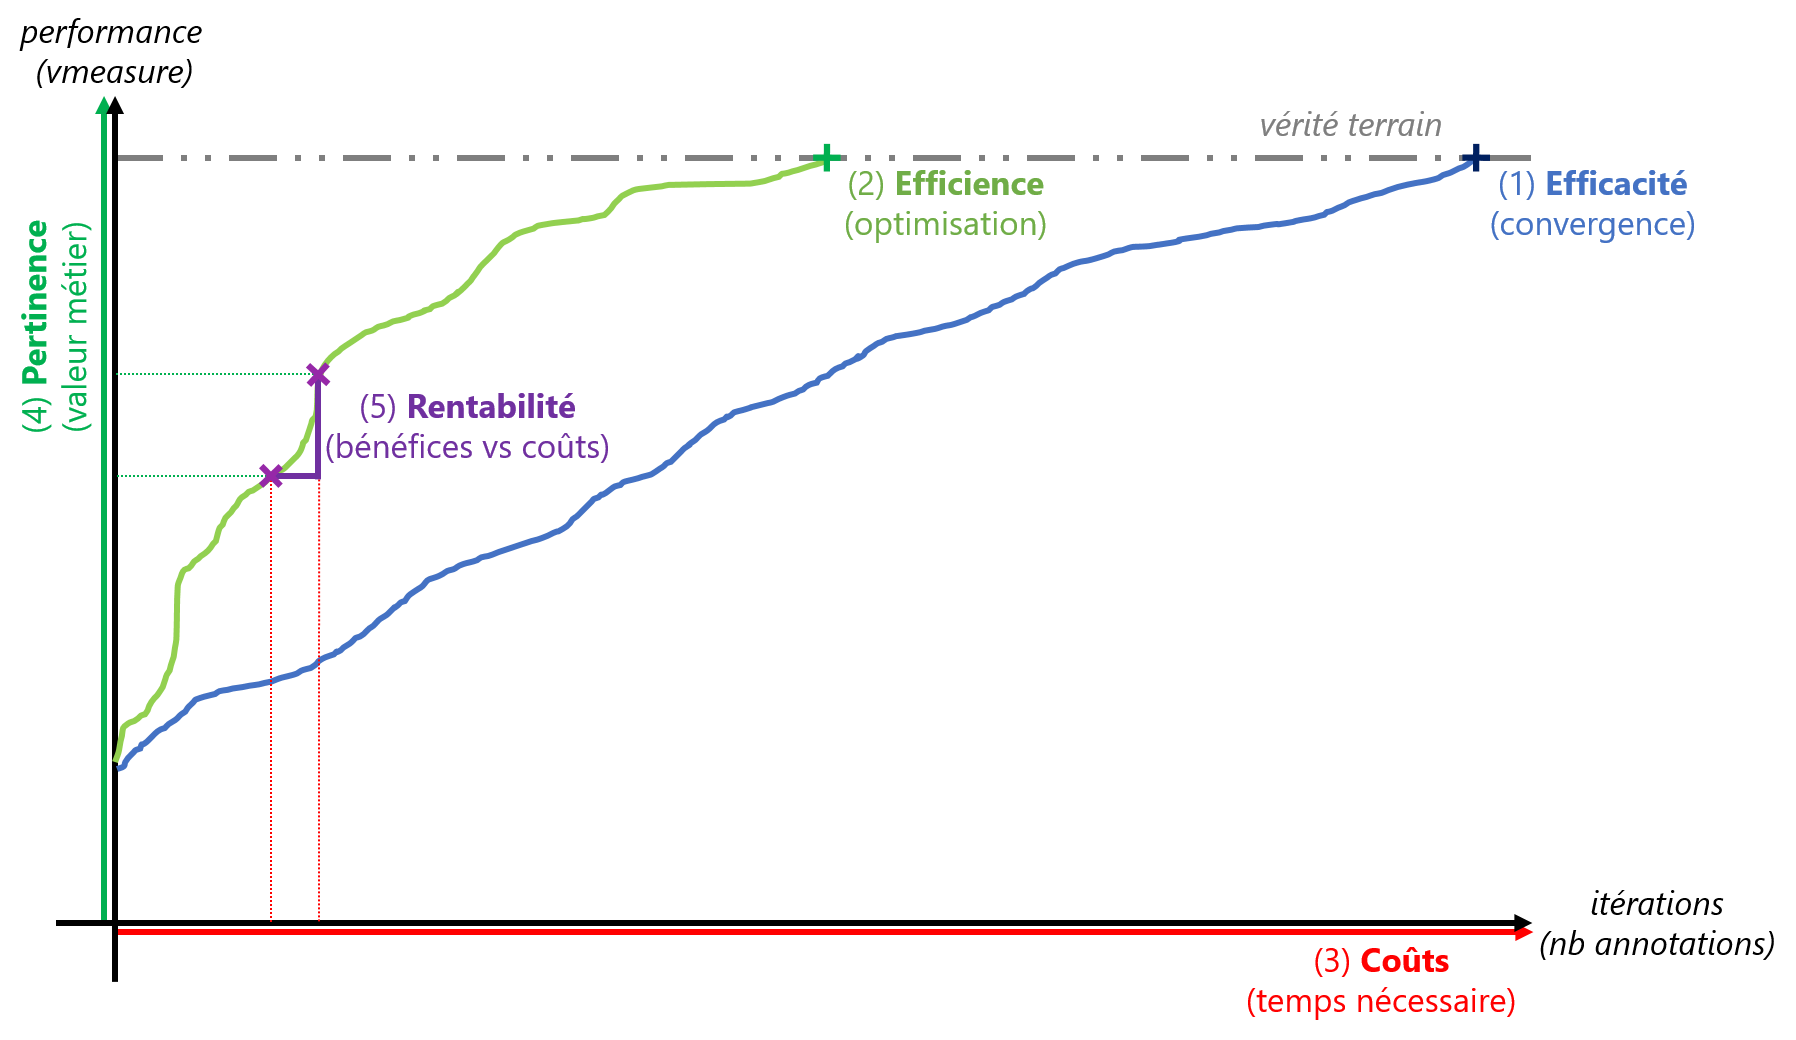
\includegraphics[width=0.95\textwidth]{figures/hypotheses-05-rentabilite}
			\caption{Illustration des études réalisées sur le \textit{clustering} interactif (\textit{étape 5/6}) en schématisant l'évolution de la performance (\textit{accord avec la vérité terrain calculé en v-measure}) d'une base d'apprentissage en cours de construction en fonction du nombre d'itérations de la méthode (\textit{nombre d'annotations par un expert métier}).}
			\label{figure:4.5-HYPOTHESE-RENTABILITE}
		\end{figure}

	\end{tcolorbox}
	
	%%%
	%%% Subsection 4.5.1: Étude d'estimation des cas d'arrêts de la méthode
	%%%
	\subsection{Étude d'estimation des cas d'arrêts de la méthode}
	
		%%% Protocole expérimental.
		\subsubsection{Protocole expérimental}
			\todo[inline]{Description succincte du protocole expérimental dans l'encadré d'hypothèse ?}

		%%% Résultats
		\subsubsection{Résultats obtenus}

		%%% Discussion
		\subsubsection{Discussion}